\documentclass[a4paper, 11pt]{article}
\usepackage{comment} % enables the use of multi-line comments (\ifx \fi) 
\usepackage{lipsum} %This package just generates Lorem Ipsum filler text. 
\usepackage{fullpage} % changes the margin
\usepackage[a4paper, total={7in, 10in}]{geometry}
\usepackage{comment} % enables the use of multi-line comments (\ifx \fi) 
\usepackage{lipsum} %This package just generates Lorem Ipsum filler text. 
\usepackage{fullpage} % changes the margin
\usepackage{ocgx}
\usepackage[fleqn]{amsmath}
\usepackage{amssymb,amsthm}  % assumes amsmath package installed
\newtheorem{theorem}{Theorem}
\newtheorem{corollary}{Corollary}
\usepackage{graphicx}
\usepackage{tikz}
\usetikzlibrary{arrows}
\usepackage{verbatim}
\usepackage[numbered]{mcode}
\usepackage{tikz}
\usepackage[fleqn]{amsmath}
\usepackage{amssymb,amsthm}  % assumes amsmath package installed
\usepackage{graphicx}
\usepackage{tikz}
\usetikzlibrary{arrows}
\usepackage{verbatim}
\usepackage[numbered]{mcode}
\usepackage{float}
\usepackage{tikz}
    \usetikzlibrary{shapes,arrows}
    \usetikzlibrary{arrows,calc,positioning}

    \tikzset{
        block/.style = {draw, rectangle,
            minimum height=1cm,
            minimum width=1.5cm},
        input/.style = {coordinate,node distance=1cm},
        output/.style = {coordinate,node distance=4cm},
        arrow/.style={draw, -latex,node distance=2cm},
        pinstyle/.style = {pin edge={latex-, black,node distance=2cm}},
        sum/.style = {draw, circle, node distance=1cm},
    }
\usepackage{xcolor}
\usepackage{mdframed}
\usepackage{enumitem}
\usepackage{indentfirst}
\usepackage{hyperref}
\usepackage{amsmath,amsthm,amsfonts,amssymb,amscd}
\usepackage{lastpage}
\usepackage{enumitem}
\usepackage{fancyhdr}
\usepackage{mathrsfs}
\usepackage{xcolor}
\usepackage{graphicx}
\usepackage{listings}
\usepackage{hyperref}
\usepackage[spanish]{babel}
\usepackage[T1]{fontenc}
\usepackage[utf8]{inputenc}
\usepackage{lipsum}
\usepackage{ragged2e}
\usepackage[makeroom]{cancel}
\usepackage{enumerate}    
\usepackage{xcolor}
\usepackage{mdframed}
\usepackage{enumitem}
\usepackage{indentfirst}
\usepackage{hyperref}
\usepackage{amsmath,amsthm,amsfonts,amssymb,amscd}
\usepackage{cancel}
\usepackage{lastpage}
\usepackage{enumitem}
\usepackage{fancyhdr}
\usepackage{mathrsfs}
\usepackage{xcolor}
\usepackage{graphicx}
\usepackage{listings}
\usepackage{hyperref}
\usepackage[english]{babel}
\usepackage[utf8]{inputenc}
\usepackage{lipsum}
\usepackage{ragged2e}
\usepackage[makeroom]{cancel}
\usepackage{listings}
    
\renewcommand{\thesubsection}{\thesection.\alph{subsection}}

\newenvironment{problem}[2][Problema]
    { \begin{mdframed}[backgroundcolor=gray!20] \textbf{#1 #2} \\}
    {  \end{mdframed}}

\newenvironment{instructions}[2][Instrucciones]
    { \begin{mdframed}[backgroundcolor=gray!20] \textbf{#1 #2} \\}
    {  \end{mdframed}}
% Define solution environment
\newenvironment{solution}
    {\textit{Solución:}}
    {}

\renewcommand{\qed}{\quad\qedsymbol}
\newcommand{\dif}[1]{\mathrm{d}y_{#1}}
\begin{document}

\noindent
%%%%%%%%%%%%%%%%%%%%%%%%%%%%%%%%%%%%%%%%%%%%%%%%%%%%%%%%%%%%%%%%%%%%%%%%%%%%%%%%%%%%%%%%%%%%%%%%%%%%%%%%%%%%%%%%%%%%%%%%%%%%%%%%%%%%%%%%
\large\textbf{Estuardo Menéndez \quad (18072) } \hfill \textbf{Proyecto \#2}   \\
\large\textbf{Lorena Beltrán \quad \qquad (18629)} \hfill \textbf{Grupo: Booleano} \\
\large\textbf{Roberto Castillo \quad \qquad(18546)} \\
\normalsize Curso: Lógica Matemática \hfill Segundo Semestre 2020\\
Instructor: Paulo Mejía \hfill Fecha de Entrega: $21$ de septiembre del 2020 \\
\noindent\rule{7in}{1pt}
 % 1. Descripción de los nodos y relaciones seleccionados
 % 2. Script  con  las  instrucciones
 % 3.Archivos  de  las  respuestas  de  las consultas, donde se evidencia    el gráfico del grafo. 
\section*{Descripción}
Los deportes son una de las áreas en donde los grafos son utilizados más ampliamente. Cualquier aficionado sueña con predecir cuales serán los resultados de un partido en particular, pero esto no es siempre fácil de predecir. Utilizando datos históricos se pueden tener predicciones que, si bien no son precisas en todos los casos, dan una idea general bastante buena de los posibles resultados. En el presente proyecto se trabaja con las estadísticas de los equipos de la NBA para predecir los resultados de los playoffs del año 2020, así como proveer al usuario de información relevante sobre sus equipos favoritos o de interes. \\
El programa, desarrollado en Neo4j (versión 4.1.0) hace uso de 3 tipos de nodos, los cuales son: 
\begin{enumerate}
    \item Equipo
    \begin{enumerate}
        \item Oeste
        \item Este
    \end{enumerate}
    \item Partido
\end{enumerate}
En este caso, los partidos tienen asignado un año y tipo (primer partido, semifinal de conferencia, final de conferencia, gran final) mientras que el equipo tiene nombre y acrónimo. La relación que se trabajó fue la de ganar, la cual representa, para un partido en particular, cuantas veces el equipo ganó.
\section*{Script de instrucciones}
Adicional al código con la creación de los equipos y partidos, se hicieron las siguientes instrucciones para analizar los datos dados e intentar predecir los resultados del partido que se está jugando actualmente (L.A. Lakers contra Denver Nuggets). El codigo para la creación de nodos puede ser enccontrado en el siguiente link: \url{https://github.com/EstuardoMenendez/ProyectoLogica2}
\begin{lstlisting}[language=SQL]
//Codigo para mostrar la historia de un equipo en particular en los playoffs.
MATCH (t:Team {Name: "Golden State"})-[w:WIN]->(:Playoff)<-[l:WIN]-()
RETURN t,w,l

//Codigo para mostrar una tabla con las estadisticas generales de los equipos
MATCH (t:Team)-[w:WIN]->(:Playoff)<-[l:WIN]-()
RETURN t.Name AS TEAM, SUM(w.Win) AS TOTAL_WIN, SUM(l.Win) AS TOTAL_LOSS,
(toFloat(SUM(w.Win)) / (toFloat(SUM(w.Win))+ toFloat(SUM(l.Win)))) AS WIN_PERCENTAGE
ORDER BY SUM(w.Win) DESC

//Codigo para mostrar el grafo del camino mas corto entre dos equipos
MATCH (t1:Team {Name: "L.A. Lakers"}),(t2:Team {Name:"Denver"}),
    p = AllshortestPaths((t1)-[*..14]-(t2))
RETURN p

//Codigo para sacar la ventaja que tendra un equipo sobre considerando el camino mas corto
MATCH p= AllShortestPaths((t1:Team {Name: "L.A. Lakers"})-[:WIN*0..14]-(t2:Team {Name:"Denver"}))
WITH [r IN relationships(p)| r.Win] AS RArray, LENGTH(p)-1  AS s
RETURN AVG(REDUCE(x = 0, a IN [i IN range(0,s) WHERE i % 2 = 0 | RArray[i] ] | x + a)) //total win
- AVG(REDUCE(x = 0, a IN [i IN range(0,s) WHERE i % 2 <> 0 | RArray[i] ] | x + a)) //total loss
AS NET_WIN
\end{lstlisting}
\\
\section*{Consultas}
\begin{figure}[h!]
        \centering
        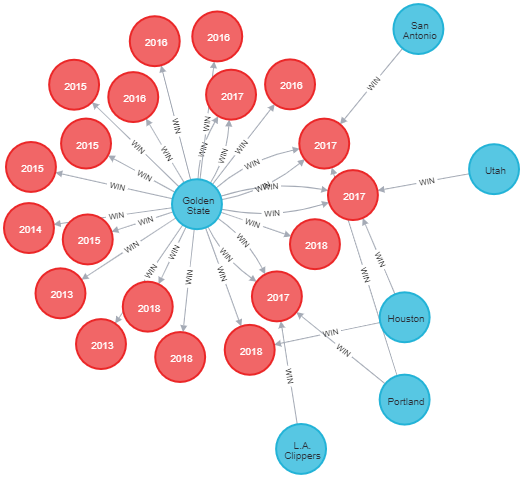
\includegraphics[width=3in]{GoldenState.png}
        \caption{Grafo de todos los nodos que se relacionan con el equipo Golden State}
\end{figure}
\begin{figure}[h!]
        \centering
        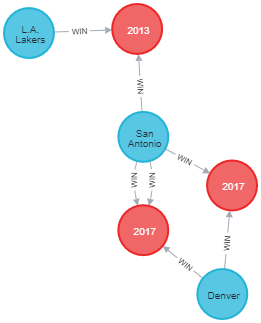
\includegraphics[width=3in]{LakersGraph.png}
        \caption{Grafo de camino más corto entre Denver y Lakers}
\end{figure}
\begin{thebibliography}{1} %% REFERENCIAS
\bibitem{ref1} Rossen, K. (2007). \textit{Discrete Mathematics and its applications, seventh edition}.New York, U.S.: McGraw-Hill Companies, Inc.
\end{thebibliography}
\end{document}
